\documentclass[10pt]{article}
\usepackage[polish]{babel}
\usepackage[utf8]{inputenc}
\usepackage[T1]{fontenc}
\usepackage{graphicx}
\usepackage[export]{adjustbox}
\graphicspath{ {./images/} }
\usepackage{amsmath}
\usepackage{amsfonts}
\usepackage{amssymb}
\usepackage[version=4]{mhchem}
\usepackage{stmaryrd}

\title{PRÓBNY EGZAMIN MATURALNY \\
 Z MATEMATYKI }

\author{}
\date{}


\begin{document}
\maketitle
\begin{center}

\includegraphics[max width=\textwidth]{2024_11_21_b8ac5f500a5bbb1b4ec5g-01(1)}
\end{center}

PESEL\\
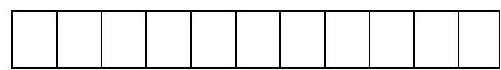
\includegraphics[max width=\textwidth, center]{2024_11_21_b8ac5f500a5bbb1b4ec5g-01}

\section*{POZIOM PODSTAWOWY}
\begin{enumerate}
  \item Sprawdź, czy arkusz egzaminacyjny zawiera 18 stron (zadania 1-34). Ewentualny brak zgłoś przewodniczącemu zespołu nadzorującego próbny egzamin.
  \item Rozwiązania zadań i odpowiedzi wpisuj w miejscu na to przeznaczonym.
  \item Odpowiedzi do zadań zamkniętych (1-25) przenieś na kartę odpowiedzi, zaznaczając je w części karty przeznaczonej dla zdającego. Zamaluj ■ pola do tego przeznaczone. Błędne zaznaczenie otocz kółkiem i zaznacz właściwe.
  \item Pamiętaj, że pominięcie argumentacji lub istotnych obliczeń
\end{enumerate}

Marzec 2018

Czas pracy:\\
170 minut

Liczba punktów do uzyskania: 50\\
w rozwiązaniu zadania otwartego (26-34) może spowodować, że za to rozwiązanie nie będziesz mógł dostać pełnej liczby punktów.\\
5. Pisz czytelnie i używaj tylko długopisu lub pióra z czarnym tuszem lub atramentem.\\
6. Nie używaj korektora, a błędne zapisy wyraźnie przekreśl.\\
7. Pamiętaj, że zapisy w brudnopisie nie będą oceniane.\\
8. Możesz korzystać z zestawu wzorów matematycznych, cyrkla i linijki oraz kalkulatora.\\
9. Na karcie odpowiedzi wpisz swój numer PESEL.\\
10. Nie wpisuj żadnych znaków w części przeznaczonej dla egzaminatora.

\section*{ZADANIA ZAMKNIĘTE}
W zadaniach od 1. do 25. wybierz i zaznacz na karcie odpowiedzi poprawna odpowiedź.

\section*{Zadanie 1. (0-1 pkt)}
Narty w styczniu kosztowały \(640 \mathrm{zł}\). W lutym obniżono ich cenę o \(25 \%\), a w marcu jeszcze o 10\%. Cena nart po drugiej obniżce jest równa:\\
A. 416 zl\\
B. 432 zl\\
C. \(605 \mathrm{zł}\)\\
D. \(553,50 \mathrm{zł}\)

\section*{Zadanie 2. (0-1 pkt)}
Wykres funkcji liniowej \(f(x)=-22 x+120\) przechodzi przez ćwiartki układu współrzędnych\\
A. I, II, III\\
B. I, II, IV\\
C. I, III, IV\\
D. II, III, IV

\section*{Zadanie 3. (0-1 pkt)}
Funkcja, której wykres przedstawiono na rysunku, jest rosnąca w przedziałach:\\
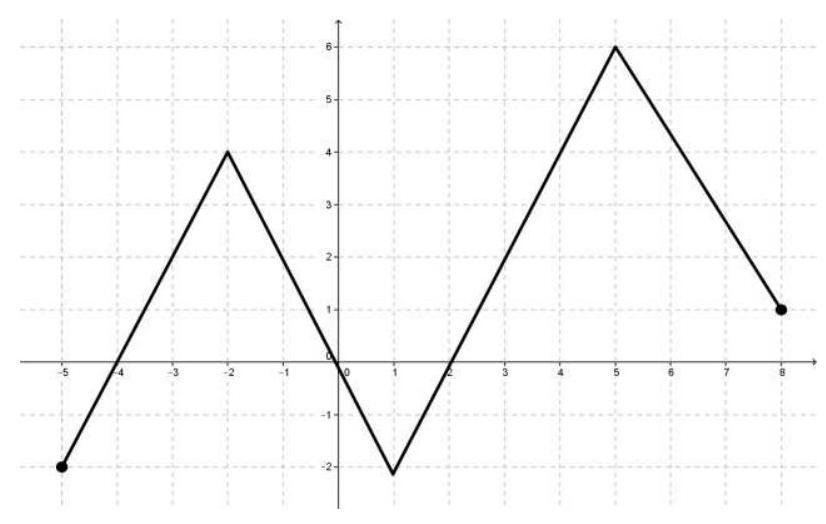
\includegraphics[max width=\textwidth, center]{2024_11_21_b8ac5f500a5bbb1b4ec5g-02}\\
A. \(\langle-2,1\rangle\) oraz \(\langle 5,8\rangle\)\\
B. \(\langle-2,1\rangle \cup\langle 5,8\rangle\)\\
C. \(\langle-5,-2\rangle\) oraz \(\langle 1,5\rangle\)\\
D. \(\langle-5,-2\rangle \cup\langle 1,5\rangle\)

\section*{Zadanie 4. (0-1 pkt)}
Ciąg \(\left(a_{n}\right)\) jest określony wzorem \(a_{n}=(-2)^{n} \cdot\left(4-n^{2}\right)\), dla \(n \geq 1\). Wtedy\\
A. \(a_{3}=40\)\\
B. \(a_{3}=-8\)\\
C. \(a_{3}=-40\)\\
D . \(a_{3}=-30\)

\section*{Zadanie 5. (0-1 pkt)}
Cosinus kąta ostrego jest równy \(\frac{\sqrt{7}}{3}\). Tangens tego kąta jest równy:\\
A. \(\frac{\sqrt{2}}{3}\)\\
B. \(\frac{\sqrt{14}}{2}\)\\
C. \(\frac{2 \sqrt{7}}{7}\)\\
D. \(\frac{\sqrt{14}}{7}\)

\section*{BRUDNOPIS}
\begin{center}

\includegraphics[max width=\textwidth]{2024_11_21_b8ac5f500a5bbb1b4ec5g-03}
\end{center}

\section*{Zadanie 6. (0-1 pkt)}
Funkcja kwadratowa, której fragment wykresu przedstawiono na rysunku, ma wzór:\\
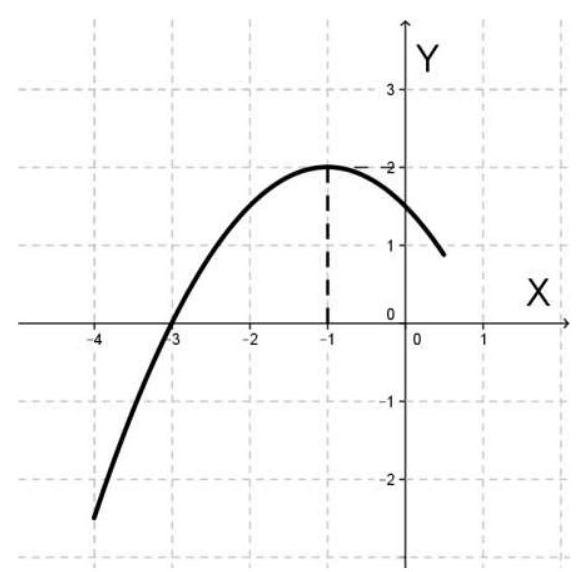
\includegraphics[max width=\textwidth, center]{2024_11_21_b8ac5f500a5bbb1b4ec5g-04(3)}\\
A. \(f(x)=-\frac{1}{2} x^{2}+x+\frac{3}{2}\)\\
B. \(\quad f(x)=-\frac{1}{2} x^{2}+x-\frac{3}{2}\)\\
C. \(f(x)=-\frac{1}{2} x^{2}-x-\frac{3}{2}\)\\
D. \(f(x)=-\frac{1}{2} x^{2}-x+\frac{3}{2}\)

\section*{Zadanie 7. (0-1 pkt)}
Wartość wyrażenia \(\frac{4 \cdot 5^{0.75}+5^{0.75}}{0,125^{\frac{-2}{3}}+5^{0}}\) jest równa:\\
A. \(5^{0.75}\)\\
B. \(5^{1,5}\)\\
C. \(2 \cdot 5^{0,75}\)\\
D. \(5 \cdot 5^{0,75}\)

\section*{Zadanie 8. (0-1 pkt)}
Ilustracja graficzna układu równań \(\left\{\begin{array}{l}2 x-y=4 \\ x+2 y=7\end{array}\right.\) jest przedstawiona na rysunku:\\
A.\\
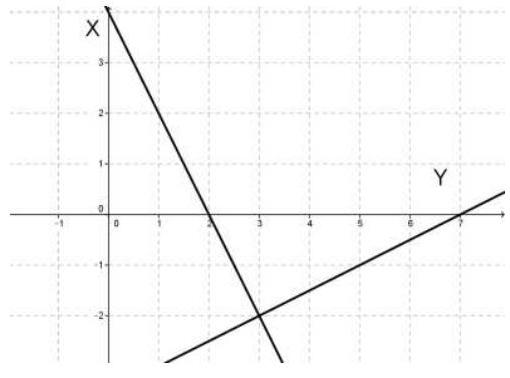
\includegraphics[max width=\textwidth, center]{2024_11_21_b8ac5f500a5bbb1b4ec5g-04(2)}\\
B.\\
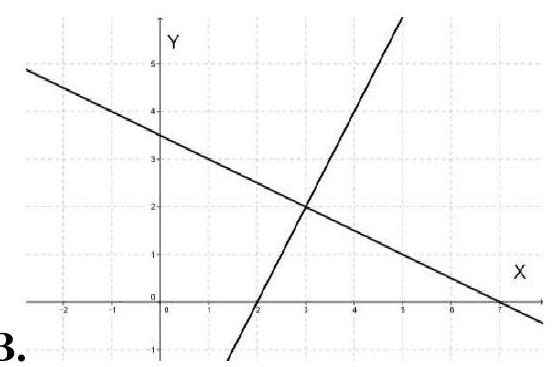
\includegraphics[max width=\textwidth, center]{2024_11_21_b8ac5f500a5bbb1b4ec5g-04(1)}\\
C.\\
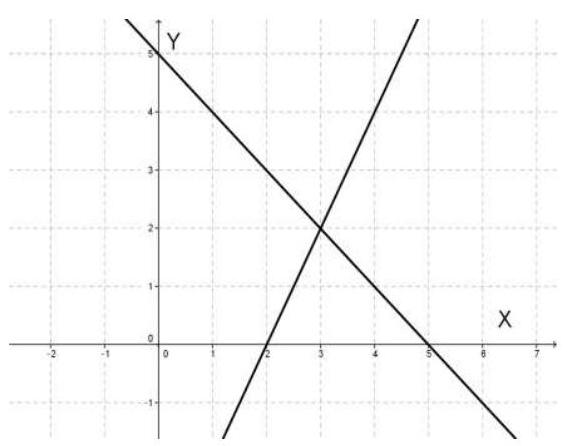
\includegraphics[max width=\textwidth, center]{2024_11_21_b8ac5f500a5bbb1b4ec5g-04}\\
D.\\
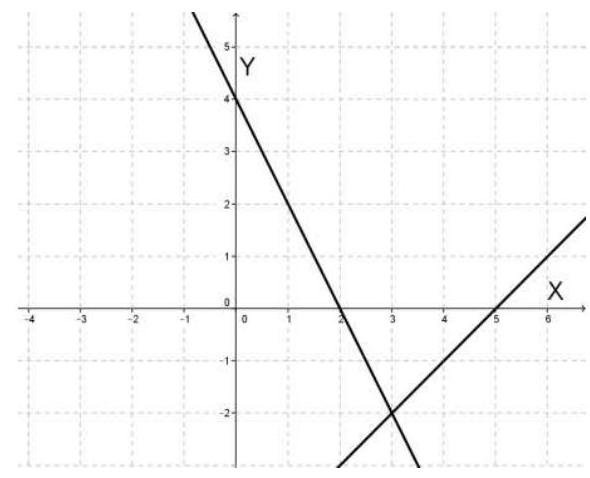
\includegraphics[max width=\textwidth, center]{2024_11_21_b8ac5f500a5bbb1b4ec5g-04(4)}

\section*{BRUDNOPIS}
\begin{center}

\includegraphics[max width=\textwidth]{2024_11_21_b8ac5f500a5bbb1b4ec5g-05}
\end{center}

\section*{Zadanie 9. (0-1 pkt)}
Iloczyn wszystkich rozwiązań równania \(\left(x^{2}+4\right)\left(x^{2}-1\right)(4 x+1)=0\) jest równy\\
A. -1\\
B. \(-\frac{1}{4}\)\\
C. \(\frac{1}{4}\)\\
D. 1

\section*{Zadanie 10. (0-1 pkt)}
Kasia w pierwszym semestrze otrzymała następujące oceny z matematyki: z prac klasowych \(3,4,4,2\), z kartkówek \(5,4,4,3,5\), z zadań domowych \(3,4,5\). Oceny z prac klasowych mają wage 5 , z kartkówek 3, z zadania domowego 2. Średnia ważona (zaokrąglona do dwóch miejsc po przecinku) ocen z matematyki Kasi w pierwszym semestrze jest równa:\\
A.3,71\\
B. 4,6\\
C. 13,7\\
D. 11,41

\section*{Zadanie 11. (0-1 pkt)}
Kąt wpisany oparty na łuku równym \(\frac{5}{9}\) długości okręgu ma miarę:\\
A. \(80^{\circ}\)\\
B. \(100^{\circ}\)\\
C. \(160^{\circ}\)\\
D. \(200^{\circ}\)

\section*{Zadanie 12. (0-1 pkt)}
Proste o równaniach \(k: 3 x+4 y-2=0\) oraz \(l: y=\frac{2 m+7}{3} x+2\) są równoległe, gdy\\
A. \(m=\frac{5}{2}\)\\
B. \(m=1\)\\
C. \(m=-\frac{3}{2}\)\\
D. \(m=-\frac{37}{8}\)

\section*{Zadanie 13. (0-1 pkt)}
Liczba \(\log _{5} \frac{125}{2}+\log _{5} \frac{2}{25}-\log _{4} \frac{1}{64}\) jest równa:\\
A. -2\\
B. 1\\
C. 4\\
D. 3

\section*{Zadanie 14. (0-1 pkt)}
Obrazem odcinka \(\overline{A B}\) o końcach w punktach \(A(-5 ;-3), B(4,1)\), w symetrii względem osi OX, jest odcinek \(\overline{A_{1} B_{1}}\) o końcach w punktach:\\
A. \(A_{1}(4 ; 1), B_{1}(-5 ;-3)\)\\
B. \(A_{1}(5 ;-3), B_{1}(-4 ; 1)\)\\
C. \(A_{1}(-5 ; 3), B_{1}(4 ;-1)\)\\
D. \(A_{1}(5,3), \quad B_{1}(-4 ;-1)\)

\section*{Zadanie 15. (0-1 pkt)}
Wartość wyrażenia \(\frac{\sqrt[3]{-800}}{\sqrt[3]{100}}\) jest równa:\\
A. -2\\
B. \(-0,2\)\\
C. 2\\
D. 0,2

\section*{BRUDNOPIS}
\begin{center}

\includegraphics[max width=\textwidth]{2024_11_21_b8ac5f500a5bbb1b4ec5g-07}
\end{center}

\section*{Zadanie 16. (0-1 pkt)}
Wszystkimi rozwiązaniami równania wymiernego \(\frac{x^{2}-x-2}{x^{2}-2 x}=0\) są:\\
A. \(x \in\{-1\}\)\\
B. \(x \in\{0 ; 2\}\)\\
C. \(x \in\{-1 ; 2\}\)\\
D. \(x \in\{-1 ; 0 ; 2\}\)

\section*{Zadanie 17. (0-1 pkt)}
Tworząca stożka jest nachylona do płaszczyzny podstawy pod kątem \(35^{0}\). Miara kąta rozwarcia stożka jest równa:\\
A. \(110^{0}\)\\
B. \(55^{0}\)\\
C. \(120^{0}\)\\
D. \(130^{0}\)

\section*{Zadanie 18. (0-1 pkt)}
Funkcja liniowa przyjmuje wartości dodatnie dla \(x \in(-\infty ; 2)\), a jej wykres przecina oś \(O Y\) w punkcie \((0 ; 4)\), zatem jej wzór ma postać:\\
A. \(y=-\frac{1}{2} x+2\)\\
B. \(y=-2 x+4\)\\
C. \(y=2 x-4\)\\
D. \(y=2 x+4\)

\section*{Zadanie 19. (0-1 pkt)}
W ciągu arytmetycznym \(a_{1}=2 \sqrt{2}\) i \(a_{2}=2 \sqrt{2}+2\). Suma wyrazów od dziesiątego do czterdziestego włącznie jest równa:\\
A. \(20 \sqrt{2}+90\)\\
B. \(60 \sqrt{2}+1470\)\\
C. \(80 \sqrt{2}+1560\)\\
D. \(62 \sqrt{2}+1488\)

\section*{Zadanie 20. (0-1 pkt)}
Punkt \(P=(-4,3)\) leży na końcowym ramieniu kąta \(\alpha\). Cosinus kąta \(\alpha\) jest równy:\\
A. \(\frac{4}{5}\)\\
B. \(-\frac{4}{5}\)\\
C. \(\frac{3}{5}\)\\
D. \(-\frac{3}{5}\)

\section*{Zadanie 21. (0-1 pkt)}
Liczb naturalnych sześciocyfrowych podzielnych przez 5, których cyfra setek należy do zbioru \(\{3,4,7,9\}\) i wszystkie cyfry są różne jest:\\
A. \(8 \cdot 7 \cdot 6 \cdot 4 \cdot 5 \cdot 2\)\\
B. \(8 \cdot 7 \cdot 6 \cdot 4 \cdot 5 \cdot 1+7 \cdot 7 \cdot 6 \cdot 4 \cdot 5 \cdot 1\)\\
C. \(9 \cdot 10 \cdot 10 \cdot 4 \cdot 10 \cdot 2\)\\
D. \(8 \cdot 8 \cdot 7 \cdot 4 \cdot 6 \cdot 1+9 \cdot 8 \cdot 7 \cdot 4 \cdot 6 \cdot 1\)

\section*{BRUDNOPIS}
\begin{center}

\includegraphics[max width=\textwidth]{2024_11_21_b8ac5f500a5bbb1b4ec5g-09}
\end{center}

\section*{Zadanie 22. (0-1 pkt)}
Wykres funkcji \(f(x)=\left(\frac{1}{2}\right)^{x-3}\) jest przedstawiony na rysunku:\\
A.\\
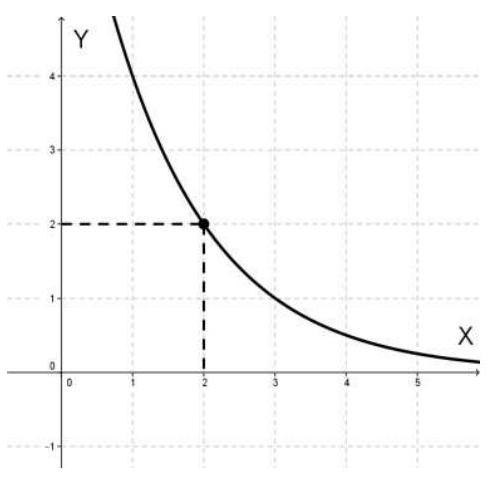
\includegraphics[max width=\textwidth, center]{2024_11_21_b8ac5f500a5bbb1b4ec5g-10(3)}\\
B.\\
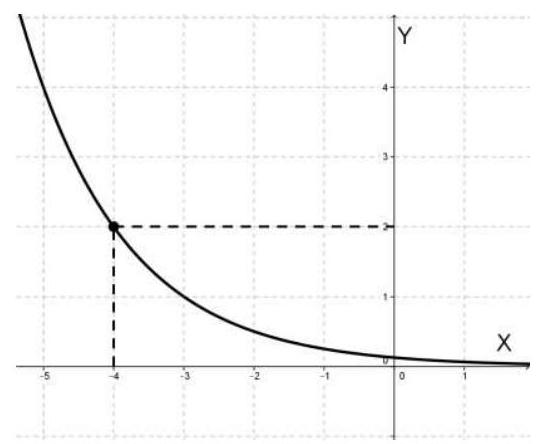
\includegraphics[max width=\textwidth, center]{2024_11_21_b8ac5f500a5bbb1b4ec5g-10(1)}\\
C.\\
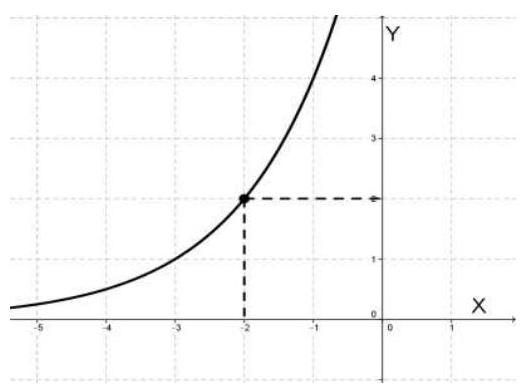
\includegraphics[max width=\textwidth, center]{2024_11_21_b8ac5f500a5bbb1b4ec5g-10}\\
D.\\
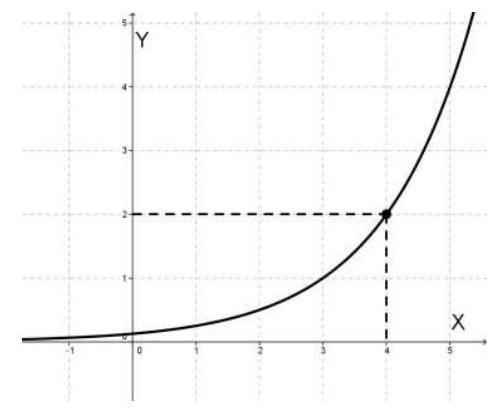
\includegraphics[max width=\textwidth, center]{2024_11_21_b8ac5f500a5bbb1b4ec5g-10(2)}

\section*{Zadanie 23. (0-1 pkt)}
Wartość wyrażenia \((2-3 \sqrt{2})^{2}\) jest równa\\
A. 22\\
B. \(22-12 \sqrt{2}\)\\
C. \(4+24 \sqrt{2}\)\\
D. \(22+12 \sqrt{2}\)

\section*{Zadanie 24. (0-1 pkt)}
Miara kąta między bokiem \(A B\) równoległoboku \(A B C D\), a przekątną \(A C\) jest równa \(30^{\circ}\). Długość przekątnej \(A C\) jest równa 5, a długość boku \(A B\) wynosi 4, zatem pole równoległoboku jest równe:\\
A. \(P=12\)\\
B. \(P=10 \sqrt{3}\)\\
C. \(P=20\)\\
D. \(P=10\)

\section*{Zadanie 25. (0-1 pkt)}
Największą wartością funkcji kwadratowej \(f(x)=-\frac{1}{3} x^{2}+4 x+1 \mathrm{w}\) przedziale \(\langle-1 ; 5\rangle\) jest\\
A. -35\\
B. \(\frac{11}{3}\)\\
C. \(\frac{38}{3}\)\\
D. 13

\section*{BRUDNOPIS}
\begin{center}

\includegraphics[max width=\textwidth]{2024_11_21_b8ac5f500a5bbb1b4ec5g-11}
\end{center}

\section*{ZADANIA OTWARTE}
Rozwiazania zadań o numerach od 26. do 34. należ̀y zapisać w wyznaczonych miejscach pod treścia zadania.

\section*{Zadanie 26. (0-2 pkt)}
Rozwiąż nierówność \((x+5)(3-x)+2 x-6 \geq 0\).\\

\includegraphics[max width=\textwidth, center]{2024_11_21_b8ac5f500a5bbb1b4ec5g-12}\\

\includegraphics[max width=\textwidth, center]{2024_11_21_b8ac5f500a5bbb1b4ec5g-12(1)}

Odpowiedź:

\section*{Zadanie 27. (0-2 pkt)}
W trójkącie równobocznym \(A B C\) połączono środki wysokości otrzymując trójkąt \(P Q R\). Wykaż, że stosunek pola trójkąta \(P Q R\) do pola trójkąta \(A B C\) jest równy \(\frac{1}{16}\).\\
\(\qquad\)

\section*{Zadanie 28. (0-2 pkt)}
Wyznacz wzór ogólny ciągu geometrycznego wiedząc, że \(a_{5}=\frac{3}{16}\) oraz \(q^{4}=-\frac{2}{3} a_{6}\).\\
\(\qquad\)\\
Odpowiedź:

\section*{Zadanie 29. (0-2 pkt)}
Udowodnij, że jeżeli przy dzieleniu przez 5 liczba całkowita \(x\) daje resztę 2, a liczba całkowita \(y\) daje resztę 3 , to iloczyn liczb \(x\) i \(y\) przy dzieleniu przez 5 daje resztę 1 .\\
\(\qquad\)

\section*{Zadanie 30. (0-2 pkt)}
Wyznacz równanie symetralnej odcinka \(A B\), gdzie \(A=(-3,4), B=(2,-1)\).\\
\(\qquad\)\\
Odpowiedź:

\section*{Zadanie 31. (0-2 pkt)}
Ze zbioru liczb \(\{1,2,3,4,5,6,7\}\) losujemy kolejno dwa razy po jednej liczbie bez zwracania. Oblicz prawdopodobieństwo zdarzenia \(A\) polegającego na tym, że pierwsza z wylosowanych liczb jest nieparzysta, a ich iloczyn jest większy od 10.\\

\includegraphics[max width=\textwidth, center]{2024_11_21_b8ac5f500a5bbb1b4ec5g-14}

Odpowiedź:

\section*{Zadanie 32. (0-4 pkt)}
Dane dwa okręgi o środkach B i C są styczne zewnętrznie i jednocześnie są styczne wewnętrznie do okręgu o środku w punkcie A. Wiedząc, że \(|B C|=|A C|\) oraz promień okręgu o środku \(C\) ma długość \(r_{c}=3\) oblicz długość odcinka AB.\\
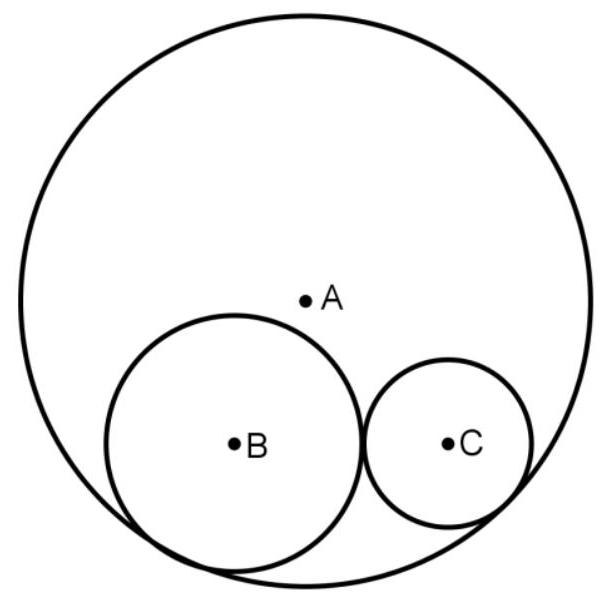
\includegraphics[max width=\textwidth, center]{2024_11_21_b8ac5f500a5bbb1b4ec5g-15}\\

\includegraphics[max width=\textwidth, center]{2024_11_21_b8ac5f500a5bbb1b4ec5g-15(1)}

Odpowiedź:

\section*{Zadanie 33. (0-5 pkt)}
Czworokąt \(A B C D\) jest trapezem równoramiennym, który nie jest równoległobokiem. Wiedząc, że podstawami trapezu są odcinki \(A B\) oraz \(C D\), przy czym \(A=(-2 ;-4)\), \(B=(7 ; 5)\) i \(D=(-1 ; 2)\), oblicz pole oraz obwód tego trapezu.\\

\includegraphics[max width=\textwidth, center]{2024_11_21_b8ac5f500a5bbb1b4ec5g-16}

Odpowiedź:

\section*{Zadanie 34. (0-4 pkt)}
Podstawą ostrosłupa jest prostokąt, którego stosunek długości boków wynosi 2:3. Pole podstawy ostrosłupa jest równe \(24 \mathrm{~cm}^{2}\). Każda krawędź boczna jest nachylona do płaszczyzny podstawy pod kątem \(\alpha=30^{\circ}\). Oblicz pole powierzchni bocznej tego ostrosłupa.\\

\includegraphics[max width=\textwidth, center]{2024_11_21_b8ac5f500a5bbb1b4ec5g-17}

Odpowiedź:

\section*{BRUDNOPIS}
\begin{center}

\includegraphics[max width=\textwidth]{2024_11_21_b8ac5f500a5bbb1b4ec5g-18}
\end{center}


\end{document}